\clearpage
\section[Nonadic compression and circular moments of the Weil form]{Nonadic compression and\\circular moments of the Weil form}
\label{sec:transporte-momentos}
\label{tm-add-seccion}

The relation between memory and positivity requires preserving two levels of readout.
A nonadic winding records a history and admits a positive Hilbert-space
realization; the arithmetic readouts of that same genealogy express a Hermitian
form involving the gamma, prime, and polar channels jointly.
The transport problem consists in identifying their energies and correlations,
with the same domains and without replacing one of these realizations by the other.
The following identities make this comparison explicit before applying
the Gelfand--Naimark--Segal (GNS) construction to the arithmetic form.

The complete balance of a nine-phase chart is preserved first, including
any norm variation at the seam. Next, the loss register,
its moment matrices, and a Cayley operator acting on exponentially
decaying test functions are constructed. Local coercivity can be transported
to entire collections of test functions with tails; passage to their algebraic sum and the global
domain additionally requires the mixed correlations specified below.
This development does not assert that global Weil positivity has been established.

% Procedencia y alcance editorial íntegros de las cabeceras originales:
% # Costura nonádica, balance de memoria y transporte de la positividad
% 
% Desarrollo focal del 11 de septiembre de 2026. No modifica las ediciones PDF entregadas. Procedencia: arquitectura autoral preexistente; formalización reunida de las identidades de compresión, con una extensión explícita al caso en que aún se comprueba la isometría de la costura. No se atribuye prioridad histórica a estas identidades operatorias.
% 
% # Momentos circulares antes de GNS: memoria nonádica y forma aritmética completa
% 
% Nota independiente de investigación matemática, 11 de septiembre de 2026.
% No modifica un PDF, un índice ni un certificado de publicación. El resultado
% propio es la composición explícita de dos construcciones anteriores a GNS:
% un núcleo positivo de memoria y unos momentos circulares de la forma completa.
% Su identificación no se presupone.
%

% SOURCE c L5-20
\subsection{Enriched state and modes of the central chart}
\label{tm-add-c1}
The construction used is APP → TRIT → TPK → enriched state → joint discrete structure of the continuum. APP preserves sum and product evaluations, their quotients and residues, on the same support. The TRIT preserves orientation and regime; the TPK composes selection, transport, and memory update. Nonadic holonomy returns the phase and increases the depth of the history. The five correlative aspects of the continuum are neither separated nor redefined through the spectral question studied subsequently.

This development begins with the realization of the winding register of that structure. It does not seek to replace the complete construction of the continuum with a sequence space. Integer memory is one coordinate of the state, not its entirety. Nor does it identify the reduced phase register with the TPK generator.

The author's note on sum and product indicates the provenance of the central matrix. In the preserved positive chart, one obtains

\[
B_c=\begin{pmatrix}7&2\\2&7\end{pmatrix}
=9P_++5P_-,\qquad
P_\pm=\frac12\begin{pmatrix}1&\pm1\\\pm1&1\end{pmatrix}.
\]
Thus, after normalization of the uniform mode, the differential mode has ratio \(q=5/9\). The names “sum” and “product” describe the APP operations generating the chart; the projectors \(P_+\) and \(P_-\) are its symmetric and antisymmetric modes. Equality between a mode and a particular sheet requires preserving the map relating them.


% SOURCE c L21-70
\subsection{Uniform compression of the nonadic chart and exact balance}
\label{tm-add-c2}
Let \(\mathcal K\) be a Hilbert space and \(C\) a bounded operator on it. On \(\mathcal K^9\), the nine-phase chart with seam \(C\) acts by

\[
S_C(v_0,\ldots,v_8)=(Cv_8,v_0,\ldots,v_7),
\qquad S_C^9=I_9\otimes C.
\]
The uniform inclusion is

\[
Jv=\frac13(v,\ldots,v),\qquad J^*J=I.
\]
Write the visible compression and its complementary component as

\[
T=J^*S_CJ=\frac{8I+C}{9},\qquad
\eta=(I-JJ^*)S_CJ.
\]
\begin{proposition}[Exact balance of compression and seam]
\label{tm-add-proposicion-costura-1}
Without assuming that \(C\) is isometric, one has

\[
\eta^*\eta=\frac8{81}(I-C)^*(I-C),
\]
\begin{equation}
\boxed{I-T^*T=\eta^*\eta+\frac19(I-C^*C).}
\label{tm-add-balance-costura}
\end{equation}
\end{proposition}

\begin{proof}
Orthogonality of \(JJ^*\) gives

\[
\eta^*\eta=J^*S_C^*S_CJ-T^*T.
\]
The first term is \((8I+C^*C)/9\). The second is \((64I+8C+8C^*+C^*C)/81\). Subtraction proves the first identity. Now subtracting \(T^*T\) from \(I\) and separating \(I-(8I+C^*C)/9\) proves \eqref{tm-add-balance-costura}.
\end{proof}

The formula does not eliminate memory: it displays exactly two contributions. One measures dispersion among the nine phases; the other measures the norm defect of the seam. If the preceding construction has given \(C^*C=I\), the positive compression–expression identity of the corpus remains:

\[
I-T^*T=\eta^*\eta\succeq0.
\]
This result explains what memory positivity contains and where identification of the readout must enter. It does not permit replacing that identification with a drawing of a circle.


% SOURCE c L71-103
\subsection{Visible contraction and preservation of the winding register}
\label{tm-add-c3}
Now suppose that \(C\) is unitary, as for the bilateral shift of integer memory. The complete winding of the differential mode is represented by \(M=qC\), not by nine successive applications of the same factor \(q\).

For each integer \(N\geq1\), define the loss-and-terminal register

\[
L_Nv=\bigl(\sqrt{1-q^2}v,
\sqrt{1-q^2}qCv,\ldots,
\sqrt{1-q^2}q^{N-1}C^{N-1}v, q^NC^Nv\bigr).
\]
\begin{proposition}[Isometric preservation of the winding register]
\label{tm-add-proposicion-costura-2}
\(L_N\) is isometric. As \(N\) increases, the last component splits into a newly expressed memory and a new terminal, without erasing the preceding register. The infinite register

\[
Lv=\left(\sqrt{1-q^2}q^jC^jv\right)_{j\geq0}
\]
is also isometric.
\end{proposition}

\begin{proof}
For \(v,w\in\mathcal K\),

\[
\langle L_Nv,L_Nw\rangle
=\left[(1-q^2)\sum_{j=0}^{N-1}q^{2j}+q^{2N}\right]
\langle v,w\rangle=\langle v,w\rangle.
\]
In the last component, \(q^NC^Nv\) is transformed into \((\sqrt{1-q^2}q^NC^Nv,q^{N+1}C^{N+1}v)\); that transformation preserves the inner product. The terminal has norm \(q^N\|v\|\), which tends to zero; the infinite sum converges and preserves the norm.
\end{proof}

For two initial states, this proof preserves their cross products; it does not merely sum energies of isolated trajectories. The positive sign of memory follows from orthogonality of its component spaces and from the isometry of the transport already constructed.


% SOURCE c L104-111
\subsection{Dual memory circle and arithmetic Cayley chart}
\label{tm-add-c4}
The integer winding register admits the bilateral shift \(Se_n=e_{n+1}\) on \(\ell^2(\mathbb Z)\). Its characters \(n\mapsto z^n\), \(|z|=1\), give the dual circle of memory. The visible phase \(r\in\{0,\ldots,8\}\) returns; the integer \(n\) is not reduced modulo \(12\) in the complete state.

If that reduction is imposed, a character descends only when \(z^{12}=1\). Thus memory without reset has a precise consequence: it permits the full circle of characters, whereas the finite calendar retains only a finite selection. This does not determine which arithmetic measure is realized on that circle.

The second circle appearing in the spectral chapter of the integral treatise is a chart of the Cayley realization. Subsection~\ref{tm-add-m4} constructs a Cayley operator directly on test functions before constructing a Hilbert space through the Weil form. Arithmetic transport can thus be compared with memory transport without introducing zero heights as inputs.


% SOURCE c L112-163
\subsubsection{Preservation of the arithmetic form under nonadic compression}
\label{tm-add-c4-1}
Arithmetic invariance of the auxiliary Cayley readout permits an additional composition. For \(a>b>1/2\), let \(C_a\) be the operator constructed in Subsection~\ref{tm-add-m4}, and let \(\mathcal T_a=(8I+C_a)/9\). The equality \(\mathscr W(C_af,C_ag)=\mathscr W(f,g)\) implies, by expansion,

\begin{equation}
\boxed{\mathscr W(f,g)=\mathscr W(\mathcal T_af,\mathcal T_ag)
+\frac8{81}\mathscr W((I-C_a)f,(I-C_a)g).}
\label{tm-add-balance-aritmetico}
\end{equation}
This identity preserves the gamma channel, prime clocks, and polar term jointly. It does not presuppose that the form is positive. The calculation consists in adding coefficients: the mixed terms have coefficients \(8\) and \(-8\), which cancel, while the two diagonal terms contribute \(72+9=81\) times the initial form. Its finite iteration gives

\begin{equation}
\mathscr W(f,g)=\mathscr W(\mathcal T_a^Nf,\mathcal T_a^Ng)
+\frac8{81}\sum_{j=0}^{N-1}
\mathscr W((I-C_a)\mathcal T_a^jf,(I-C_a)\mathcal T_a^jg).
\label{tm-add-balance-iterado}
\end{equation}
In the ordinary \(L^2\) representation, where \(C_a\) is already unitary, the same calculation is a positive norm decomposition. On the arithmetic form it is, initially, exact conservation of signed energy. The difference between these two assertions is located in a common identity; it is not hidden in a change of representation.

In a circular chart \(z=e^{i\theta}\), compression sends \(z\) to \(t(z)=(8+z)/9\). Therefore,

\[
1-|t(z)|^2=\frac8{81}|1-z|^2
=\frac{32}{81}\sin^2(\theta/2).
\]
Angular separation thus has an exact expression as complementary energy. This is the image of nonadic compression of a phase chart; the drawing does not identify it with another operator of the corpus. Nor is this map \(t(z)\) confused with the radial factor \(5/9\), which arises from the two modes of the central APP chart.

\begin{figure}[htbp]
\centering
\begin{tikzpicture}[font=\small,>=stealth]
\begin{scope}[x=1cm,y=1cm]
\draw[->,gray] (-2.35,0)--(2.65,0) node[right] {$\Re z$};
\draw[->,gray] (0,-2.2)--(0,2.25) node[above] {$\Im z$};
\draw[thick] (0,0) circle (2);
\draw[very thick] (1.777778,0) circle (.222222);
\fill (1,1.732051) circle (1.5pt) node[above right] {$z$};
\fill (1.888889,.19245) circle (1.5pt);
\draw[->] (1.10,1.57)--(1.85,.34);
\draw[dotted] (0,0)--(1,1.732051);
\draw (1.95,.20)--(2.65,.75) node[right] {$t(z)$};
\node[below] at (2,0) {$1$};
\node[above left] at (-1.30,1.4) {$|z|=1$};
\node[align=center] at (0,-2.72)
 {$t(z)=\dfrac{8+z}{9}$\\[3pt]
 $\left|t(z)-\dfrac89\right|=\dfrac19$};
\end{scope}
\begin{scope}[shift={(8,0)}]
\node[align=center] (f) at (0,1.5) {Phase representation\\[3pt] $r\longmapsto r$};
\node[align=center] (m) at (0,0) {Memory transport\\[3pt] $(r,n)\longmapsto(r,n+1)$};
\draw[->,thick] (f)--(m);
\node[draw,rounded corners,inner sep=8pt,align=center] at (0,-1.65)
 {$1-|t(z)|^2=\dfrac8{81}|1-z|^2$\\[5pt]
 Representation and complement};
\end{scope}
\end{tikzpicture}
\caption{The circular chart of nonadic compression. On the left,
the unit circle and its image with center \(8/9\) and radius \(1/9\),
drawn to the same scale; the image of \(z=e^{i\pi/3}\) is shown.
On the right, phase return is accompanied by memory advancement.
The lower balance quantifies the complementary component. This figure
represents the map \(t\), distinct from the modal factor \(q=5/9\) of the
central chart.}
\label{fig:compresion-circular}
\end{figure}


The local Schur development gives the arithmetic form a positive sign on a concrete functional domain and its transport images. Identities \eqref{tm-add-balance-aritmetico}–\eqref{tm-add-balance-iterado} do not by themselves authorize declaring all their summands positive for an arbitrary test function: they locate exactly which energies and correlations an extension of that domain must preserve.


% SOURCE c L164-190
\subsection{Criterion for transporting positivity through mixed moments}
\label{tm-add-c5}
Let \(\mathcal D\) be the common domain of the previously constructed readouts. Let \(\mathscr W\) be the sesquilinear form expressed by their gamma, prime, and polar channels. The analytic formula is received after the native generator; it does not select the seeds or preceding coefficients.

Let \(C_a\) be the reversible transport on test functions and \(S\) the memory shift. We explicitly use \(C_a(\mathcal D)=\mathcal D\) and the identity \(\mathscr W(C_af,C_ag)=\mathscr W(f,g)\), proved for the exponential class of test functions in Subsections~\ref{tm-add-m4} and~\ref{tm-add-m5}. For a collection \(\mathcal E\subset\mathcal D\), suppose a linear map \(V:\operatorname{span}\mathcal E\to\mathcal K\) has been constructed such that, for every \(f,g\) in that collection and every integer \(n\),

\begin{equation}
\boxed{\mathscr W(C_a^n f,g)=\langle S^nVf,Vg\rangle.}
\label{tm-add-criterio-momentos}
\end{equation}
\begin{proposition}[Transport of positivity by identification of moments]
\label{tm-add-proposicion-costura-3}
Identity \eqref{tm-add-criterio-momentos} implies positivity of \(\mathscr W\) on the span of the orbits \(C_a^n\mathcal E\). If that space is dense in \(\mathcal D\) for the joint norm of the readouts, and these are continuous for that norm, positivity extends to \(\mathcal D\).
\end{proposition}

\begin{proof}
For \(F=\sum_j C_a^{n_j}f_j\), invariance of \(\mathscr W\) under \(C_a\) and \eqref{tm-add-criterio-momentos} give

\[
\begin{aligned}
\mathscr W(F,F)
&=\sum_{i,j}\mathscr W(C_a^{n_i-n_j}f_i,f_j)\\
&=\left\|\sum_i S^{n_i}Vf_i\right\|^2\geq0.
\end{aligned}
\]
If a combination represents the zero function, the same identity forces the vector combination to have zero norm; the realization is well-defined. Passage to the closure uses continuity of both readouts, not a subsequent choice of sign.
\end{proof}

This is a construction criterion with explicit domains, not an assertion that \eqref{tm-add-criterio-momentos} has been proved for all readouts of the corpus. Extension from the initial collection to its orbits requires preserving all cross moments: proving it only for \(n=0\) on that initial collection does not complete the extension. Naturally, a Gram identity already proved for \(n=0\) on all of \(\mathcal D\) would directly prove positivity on that domain.


% SOURCE c L191-211
\subsection{Energy identification and two-column realization}
\label{tm-add-c6}
The corpus preserves two columns \(J_+\) and \(J_-\) and an effective analytic connector between them. It also describes a native encoding \(\Xi\) and an orthogonal projection \(P\). When the two moment identities are calculated on the same domain,

\[
\langle\Xi f,\Xi g\rangle=\langle J_+f,J_+g\rangle,
\qquad
\langle P\Xi f,P\Xi g\rangle=\langle J_-f,J_-g\rangle,
\]
subtraction gives

\begin{equation}
\mathscr W(f,g)=\langle(I-P)\Xi f,(I-P)\Xi g\rangle.
\label{tm-add-dos-columnas}
\end{equation}
The dossier calculates the uniform expectation and Helmert refinement separately. Their joint conjugation preserves both Grams and cannot, by a mere change of notation, turn a difference operator into an evaluation operator. The recovered gamma connector realizes an additional analytic operation, which must preserve its energy budget. This clarification brings together existing operations; it does not declare the TPK architecture nonexistent.

Formulas \eqref{tm-add-criterio-momentos} and \eqref{tm-add-dos-columnas} are two compatible expressions of the route to be completed: the first organizes returns and their correlations; the second organizes the visible part and complementary memory. The Schur-complement estimate in the dossier gives effective control of that energy in a complete window and all its refinements. Its scope is stated with the concrete window, without replacing the global domain by that window.


% BEGIN PROCEDENCIA COSTURA, FUENTE L212
% ## 7. Localizadores materiales y continuidad
% 
% - APP central, modos \(9/5\): `base_c01_sin_encabezado.tex`, construcción de la carta central; capítulo `78_doble_circulo_campo_espectral_completo.tex`, entorno de líneas 1276–1280.
% - Memoria anterior a la representación espectral: `cap08_holonomia_helice_memoria.tex`, especialmente la cubierta entera y la publicación \(C_{108}\).
% - Conexión y compresión–expresión: `certificados/ley_nueve_puertas_2026-07-30/DELTA_CONEXION_NONADICA_CONJUNTA_COMPRESION_EXPRESION_2026-08-16.md`, §§1–3.
% - Doble círculo y transporte cilíndrico: propietario `78_doble_circulo_campo_espectral_completo.tex`, líneas 940–1260.
% - Dos momentos nativos: propietario `10b_prueba_espectral_polar_riemann_weil_rectificacion_probatoria_20260903.tex`, líneas 235–452.
% - Propietarios completos y rutas absolutas: [recuperación conservada](../ARITMETICA_GENEALOGICA_PRIMOS_DESARROLLO_DOBLE_CIRCULO_20260911/01_HALLAZGOS_PROPIETARIOS_DOBLE_CIRCULO.md).
% 
% La selección editorial sigue siendo el integral de 2.249 páginas y sus desarrollos adyacentes. Los verificadores históricos que devuelven 2.084 páginas no cambian esa selección. Ningún control de huellas o de compilación se utiliza aquí como prueba de positividad global.
% END PROCEDENCIA COSTURA

% SOURCE m L9-53
\subsection{Operator provenance and the function of the readouts}
\label{tm-add-m1}

% BEGIN LOCALIZADORES M1
% Propietarios y localizadores de esta lectura:
% 
% - Integral autoral de 2.249 páginas, propietario
%   `output/REVISION_EDITORIAL_HMT_MD_20260905/01_FUENTES/INTEGRAL/tree/New project/output/ENSAMBLADO_CAUSAL_RESTAURADO_HMT_MD_20260905/fuente/manuscrito/integracion_83/parte_v/tex/fuentes_propietarias/editor_ready/78_doble_circulo_campo_espectral_completo.tex`.
%   Se ha releído su cuerpo completo, 1–1929, en la copia conservada en el
%   manuscrito de primos. El cociclo está en 943–968; el orden
%   positividad → GNS → Stone → Cayley, en 525–612 y 969–987; el transporte
%   cilíndrico torcido, en 1023–1118; la pérdida por vuelta, en 1171–1237;
%   la costura de nueve fases, en 1421–1495; la fórmula aritmética, en 1578–1610.
% - `output/ARITMETICA_GENEALOGICA_PRIMOS_DESARROLLO_DOBLE_CIRCULO_20260911/01_HALLAZGOS_PROPIETARIOS_DOBLE_CIRCULO.md`, leído completo. Conserva los
%   localizadores de los antecedentes del bloque APP y de la memoria anteriores
%   al GNS; no se confunde su lectura con una nueva lectura íntegra de cada
%   antecedente que cita.
% - `output/ARITMETICA_GENEALOGICA_PRIMOS_PRESENTACION_20260911/antecedentes/recuperacion_gamma/narrativa_205_paginas/CONSTANTES_ESTRUCTURA_Y_REALIDAD_FISICA_RECOPILACION_INTEGRA.md`, lectura focal 5710–5905. En 5740–5869 reúne producto nativo,
%   irreducibles, ocupaciones, calor/Mellin, canal polar y los dos círculos.
%   No ofrece allí una secuencia Toeplitz adicional anterior a GNS.
% - `output/ARITMETICA_GENEALOGICA_PRIMOS_PRESENTACION_20260911/manuscrito/03_DOBLE_CIRCULO_Y_TRANSPORTE_ESPECTRAL.md`, §§2–3, para la forma completa,
%   su continuidad y las dos columnas; en este corte se ha releído §2,
%   líneas 119–191, y se conserva el análisis anterior de §3.
% - `output/AUDITORIA_INTEGRAL_PUBLICABILIDAD_HMT_MD_20260906/COORDINACION_20260906/TRAZA_GENERATIVA_COORDINADA.md`: consulta focal de lectores espectrales;
%   desde 1524 remite a los momentos primos, no a una medida circular de Weil
%   ya seleccionada por la memoria.
% 
% La puerta del núcleo permanente y su autocomprobación causal pasaron. La
% puerta histórica `apply-hmt-first-principles` resuelve 2.084 páginas; se conserva
% como control de ese testigo, no como sustituto de la selección autoral de
% 2.249 páginas. No se afirma lectura íntegra del corpus ni del documento de 205
% páginas.
% 
% END LOCALIZADORES M1
The chain used is APP → TRIT → TPK → enriched histories of the joint continuum → arithmetic and memory readouts → circular representation. The five continuum operations remain on the same histories; this development studies a readout of their memory and does not construct an isolated fifth branch. The prime readout uses irreducibles produced by the native product; constants already expressed by HMT enter the readouts only subsequently.

\textbf{Provenance.} Cocycle, loss, two sheets, memory groups, and double circle: preexisting authorial architecture and recovered results. The assembled proofs below are a new formalization of these antecedents. No historical priority is claimed for Poisson kernels, Cayley, or Toeplitz identities. The provenance of this exact composition within the corpus has not been exhaustively investigated beyond the source owners indicated.


% SOURCE m L54-83
\subsection{Regular memory representation preceding arithmetic GNS}
\label{tm-add-m2}
The central APP block, with its symmetric and antisymmetric projectors, is

\[
B_c=\begin{pmatrix}7&2\\2&7\end{pmatrix}
=9P_++5P_-.
\]
Normalization of the differential mode expresses \(q=5/9\). A complete TPK winding preserves phase and increments integer memory:

\[
m(\Gamma_9^n)=n,\qquad
m(\gamma_2\gamma_1)=m(\gamma_2)+m(\gamma_1).
\]
On a reversible orbit of that memory, its lifted states are identified with \(e_n\), \(n\in\mathbb Z\), and the winding is the shift \(Se_n=e_{n+1}\). Injectivity of this enumeration follows from the memory increment. If one starts only from the semigroup of positive windings, the same bilateral space is the shift extension adding its predecessors; reversibility is not attributed to a transition proved only isometric. In a complete tree, the remaining labels are preserved in a transverse factor: the shift acts on memory and does not identify routes.

This \(S\) is not the Weil Cayley operator inserted into the seam. It is the regular realization of the integer memory operation. Its Hilbert-space positivity is known before forming a GNS of the arithmetic form.


% SOURCE m L84-120
\subsubsection{Loss vector, correlations, and terminal term}
\label{tm-add-m2-1}
Telescoping over windings produces weights \((1-q^2)q^{2j}\). Their amplitude in memory is the explicit vector

\[
v_q=\sqrt{1-q^2}\sum_{j=0}^{\infty}q^j e_j,
\qquad \|v_q\|^2=1.
\]
With inner product linear in the first variable, for \(n\ge0\),

\[
\langle S^n v_q,v_q\rangle
=(1-q^2)\sum_{j\ge0}q^j q^{j+n}=q^n.
\]
Conjugation and unitarity give, for every integer,

\[
\boxed{m_n^{\mathrm{mem}}=q^{|n|}.}
\]
The truncation \(v_{q,N}=\sqrt{1-q^2}\sum_{j=0}^{N-1}q^j e_j\) preserves the terminal exactly:

\[
\|v_{q,N}\|^2=1-q^{2N},\qquad
\langle S^n v_{q,N},v_{q,N}\rangle
=q^n\bigl(1-q^{2(N-n)}\bigr),\quad 0\le n<N.
\]
For \(n\ge N\), that truncated correlation is zero. Thus, for each fixed \(n\), the difference from the complete moment is \(q^{2N-n}\) when \(N>n\), and tends to zero. This formula neither erases the last register nor equates a truncation with the whole history.


% SOURCE m L121-159
\subsubsection{Triangular factorization and determinant of the memory matrices}
\label{tm-add-m2-2}
For indices \(0,\ldots,N\), define

\[
T_N=(q^{|i-j|})_{0\le i,j\le N}.
\]
It is a Gram matrix of \(v_q,Sv_q,\ldots,S^Nv_q\), so

\[
\sum_{i,j=0}^{N}\overline{c_i}c_j(T_N)_{ij}
=\left\|\sum_{j=0}^{N}c_jS^jv_q\right\|^2\ge0.
\]
There is also an exact proof without infinite series. Let

\[
L_{ij}=\begin{cases}q^{i-j},&i\ge j,\\0,&i<j,\end{cases}
\qquad D=\operatorname{diag}(1,1-q^2,\ldots,1-q^2).
\]
Then \(T_N=LDL^*\). For \(i\ge j\), the product entry is

\[
q^{i+j}+(1-q^2)\sum_{k=1}^{j}q^{i+j-2k}
=q^{i-j}.
\]
Symmetry gives the full matrix identity. A Cholesky factor is \(L D^{1/2}\), and, since \(\det L=1\),

\[
\boxed{\det T_N=(1-q^2)^N=(56/81)^N>0.}
\]
This positive kernel arises from loss and preserved memory. It requires no zeros, positive zeta function, or Weil GNS.


% SOURCE m L160-184
\subsection{Phase, nonadic refinement, and weak convergence of states}
\label{tm-add-m3}
A fixed-phase representation is obtained from

\[
v_{r,\theta}=\sqrt{1-r^2}\sum_{j\ge0}r^j e^{-ij\theta}e_j,
\quad 0<r<1,
\]
and produces \(m_n=r^{|n|}e^{in\theta}\). The Toeplitz matrices are diagonal conjugates of the preceding ones and have determinant \((1-r^2)^N\). Here the phase \(\theta\) is a coordinate of the character collection; no arithmetic spectral phase has been selected.

On the circle, with normalized Haar measure \(d\lambda\), these moments have the explicit measure

\[
d\nu_{r,\theta}(z)
=\frac{1-r^2}{|1-r e^{-i\theta}z|^2}\,d\lambda(z).
\]
Expanding both geometric series directly proves its Fourier coefficients without using a target measure.


% SOURCE m L185-219
\subsubsection{Nonadic roots of the radius and phase compatibility}
\label{tm-add-m3-1}
Taking \(r_m=q^{1/9^m}\), one has \(0<r_m<1\), \(r_{m+1}^{9}=r_m\), and \(r_m\to1\). For fixed phase,

\[
r_m^{|n|}e^{in\theta}\longrightarrow e^{in\theta}
\quad\text{for each }n\in\mathbb Z.
\]
The measures are probabilities; uniform approximation by trigonometric polynomials extends moment convergence to every continuous function. Consequently,

\[
\nu_{r_m,\theta}\ \rightharpoonup\ \delta_{e^{i\theta}}.
\]
This shows how an atomic measure can arise as a weak limit of memory states. It is not a strong limit of the vectors in the same regular representation: each coefficient of \(v_{r_m,\theta}\) tends to zero, but their norms remain one.

A naturality qualification must be preserved. Under \(p_9(z)=z^9\),

\[
(p_9)_*\nu_{r,\theta}=\nu_{r^9,9\theta}.
\]
Thus the nonadic radius with fixed phase does \textbf{not} by itself give a projective system of measures under \(p_9\). This requires retaining lifted phases with \(9\theta_{m+1}=\theta_m\pmod{2\pi}\), including their branch choices; alternatively, one must declare that the refinement used keeps the angular coordinate fixed and changes only the radius. These are different operations.


% SOURCE m L220-236
\subsubsection{State selection and change of spectral type}
\label{tm-add-m3-2}
Memory produces the group, positivity of its Grams, and these compatible correlation collections. A particular phase or a mixture of phases requires the readout selecting its amplitudes. For example, the vector \(e_0\) produces \(m_n=\mathbf1_{n=0}\); \((e_0+e_1)/\sqrt2\) produces \(m_0=1,m_{\pm1}=1/2\), with all other moments zero. The same memory operation admits both positive states.

The regular representation has vector measures absolutely continuous with respect to Haar measure. A fixed \(L^2\) vector filter cannot produce a nonzero purely atomic measure. The preceding weak limit shows a precise way for spectral type to change under refinement: that limit of states must be preserved and controlled, rather than merely increasing the length of a previously chosen phase orbit. This does not deny the spectral representation of the corpus or joint HMT generation; it distinguishes the domains of two readouts.


% SOURCE m L237-295
\subsection{Cayley operator on the exponential test-function domain}
\label{tm-add-m4}
A second object is now constructed, without assuming Weil positivity. The native product and its irreducibles already provide \(\ell_{p,k}=k\log p\), \(w_{p,k}=(\log p)p^{-k/2}\). The gamma and polar readouts complete the form \(\mathscr W\) written in Subsection~\ref{tm-add-m5}. Memory supplies an integer iteration index; the following operator acts effectively on the functions of that representation.

The operator \(C_a\) is an auxiliary analytic readout of this formalization. The choice \(a>1/2\) does not silently replace the canonical seam \(a=1/2\), nor is it declared that this choice has already been selected by the TPK.

Fix \(a>b>1/2\). Let \(\mathscr E_b\) be the space of smooth functions such that, for each derivative order \(j\), \(\sup_x e^{b|x|}|f^{(j)}(x)|<\infty\). It contains all compactly supported test functions. Define

\[
(R_a^+f)(x)=\int_0^\infty e^{-at}f(x+t)\,dt,
\qquad
(R_a^-f)(x)=\int_0^\infty e^{-at}f(x-t)\,dt,
\]
\[
\boxed{C_af=f-2aR_a^+f,\qquad C_a^{-1}f=f-2aR_a^-f.}
\]
These integrals are translation readouts constructed on the test functions; they do not use the spectrum of zeros. The parameter \(a=1\), for example, comes from the unit and allows a choice \(1/2<b<1\); it calibrates no zero.

\paragraph{Domain, inverse, and unitary realization.} The inequality \(e^{b|x|}|f(x\pm t)|\le M_0e^{bt}\) gives the bound \(\|R_a^\pm f\|_b\le\|f\|_b/(a-b)\), also for every derivative. Thus both operators preserve \(\mathscr E_b\). With the convention \(\widehat f(z)=\int f(x)e^{-izx}\,dx\), their multipliers are

\[
\widehat{C_af}(z)=c_a(z)\widehat f(z),\qquad
c_a(z)=\frac{z-ia}{z+ia},
\]
and the inverse operator has multiplier \(c_a(z)^{-1}\). The identity on the real Fourier axis proves both inverse compositions. In \(L^2\), \(|c_a(t)|=1\), so \(C_a\) is unitary for the ordinary norm, without using the Weil norm. On test functions it can be written \(C_a=(H+ia)(H-ia)^{-1}\), with \(H=i\partial_x\); here the integral formula, not a GNS generator, defines the operators.

\paragraph{Convergence condition at the polar boundary.} The parameter \(a=1/2\) of the source owner's Cayley operator cannot simply be inserted into these pre-GNS integrals. For a compactly supported test function, \(R_{1/2}^+f\) generally has a tail proportional to \(e^{x/2}\) towards \(-\infty\); its negative polar evaluation does not converge. Divergence of the assembled form has not been proved; rather, this term-by-term decomposition requires the margin \(a>1/2\). The GNS Cayley operator may subsequently use \(a=1/2\) on its Hilbert-space domain.


% SOURCE m L296-352
\subsection{Joint preservation of the gamma, prime, and polar channels}
\label{tm-add-m5}
For \(f,g\in\mathscr E_b\), let

\[
C_{f,g}(u)=\int f(x)\overline{g(x-u)}\,dx,
\qquad P_f^\pm=\int f(x)e^{\pm x/2}\,dx.
\]
The complete form is defined by

\[
\begin{aligned}
\mathscr W(f,g)={}&c_\Gamma C_{f,g}(0)
+\int_0^\infty\frac{e^{-u/2}}{1-e^{-2u}}
 [2C_{f,g}(0)-C_{f,g}(u)-C_{f,g}(-u)]\,du\\
&-\sum_{p,k}w_{p,k}
 [C_{f,g}(\ell_{p,k})+C_{f,g}(-\ell_{p,k})]\\
&+P_f^+\overline{P_g^-}+P_f^-\overline{P_g^+},
\qquad c_\Gamma=\psi(1/4)-\log\pi.
\end{aligned}
\]
\paragraph{Existence and continuity of the complete form.} The correlation bound \(|C_{f,g}(u)|\le M_fM_g(|u|+1/b)e^{-b|u|}\) proves absolute convergence of the prime sum, dominated by a series of the form \(\sum_{n\ge2}(\log n)(1+\log n)n^{-b-1/2}\). The symmetric correlation difference is \(O(u^2)\) at zero, whereas the gamma weight is \(O(u^{-1})\); at infinity the weight is exponential. Polar evaluations converge because \(b>1/2\). These bounds also prove continuity in the indicated seminorms. Positivity is not used.

\paragraph{Simultaneous invariance of the three channels.}
\label{tm-add:invariancia-weil} Since \(C_a\) is unitary on \(L^2\) and commutes with all translations,

\[
C_{C_af,C_ag}(u)=C_{f,g}(u)\qquad(u\in\mathbb R).
\]
By Fubini, the two polar readouts satisfy

\[
P_{C_af}^+=-\frac{a-1/2}{a+1/2}P_f^+,
\qquad
P_{C_af}^-=-\frac{a+1/2}{a-1/2}P_f^-.
\]
The factors are real and reciprocal, so each cross polar product is preserved exactly. Combining the three channels,

\[
\boxed{\mathscr W(C_af,C_ag)=\mathscr W(f,g).}
\]
The identity holds for all integer powers and all cross terms. It proves invariance of a Hermitian form, not its sign.


% SOURCE m L353-383
\subsection{Circular moments of the complete arithmetic form}
\label{tm-add-m6}
Define

\[
m_n^{\mathrm{ar}}(f,g)=\mathscr W(C_a^n f,g),\qquad n\in\mathbb Z.
\]
The complete formula in Subsection~\ref{tm-add-m5}, with \(C_a^nf\) in its first argument, calculates these moments from primes, gamma, and polar terms. Each evaluation exists in \(\mathscr E_b\); it requires neither a list of zeros nor a positive metric. Hermiticity and the preceding invariance give

\[
m_{-n}^{\mathrm{ar}}(g,f)=\overline{m_n^{\mathrm{ar}}(f,g)},\qquad
\mathscr W(C_a^j f,C_a^k g)=m_{j-k}^{\mathrm{ar}}(f,g).
\]
For a single test function, the matrix \(T_N^{\mathrm{ar}}(f)_{jk}=m_{k-j}^{\mathrm{ar}}(f,f)\) is Hermitian Toeplitz and satisfies the exact identity

\[
c^*T_N^{\mathrm{ar}}(f)c
=\mathscr W\!\left(\sum_{k=0}^N c_k C_a^k f,
                    \sum_{k=0}^N c_k C_a^k f\right).
\]
The matrix has been constructed without assuming positivity. The equality allows its positivity to be compared with a native memory Gram; it does not presuppose it.


% SOURCE m L384-406
\subsubsection{Polar growth and a necessary cancellation condition}
\label{tm-add-m6-1}
For \(a=1\), the exact polar contribution to \(m_n^{\mathrm{ar}}(f,g)\) is

\[
(-1/3)^nP_f^+\overline{P_g^-}
+(-3)^nP_f^-\overline{P_g^+}.
\]
For a nonzero real, even, positive test function, \(P_f^+=P_f^-=p>0\), so \(p^2[(-1/3)^n+(-3)^n]\) appears. If the total moment sequence is positive definite, its order-two minors force

\[
|m_n^{\mathrm{ar}}(f,f)|\le m_0^{\mathrm{ar}}(f,f).
\]
Thus circular identification must account for the concrete cancellation of this growth with the gamma and prime channels. Formal symmetry of the two sheets does not replace that calculation. This observation does not declare that cancellation fails; it provides an exact falsifier for a candidate composition.


% SOURCE m L407-424
\subsubsection{Mixed moment matrices and domain coverage}
\label{tm-add-m6-2}
For a collection of test functions \(f_1,\ldots,f_d\), the appropriate object is the block Toeplitz matrix

\[
\mathsf T_{(j,r),(k,s)}
=m_{k-j}^{\mathrm{ar}}(f_s,f_r).
\]
Its quadratic form is \(\mathscr W(F,F)\), where \(F=\sum_{k,s}c_{k,s}C_a^k f_s\). Controlling only the scalar matrices of some test functions does not control cross terms between different test functions. For a dense collection in each \(C_c^\infty([-R,R])\), the continuity proved above permits passage to the complete domain, provided the mixed Grams and compatibilities as \(R\) increases have been established. Increasing \(N\) along a single orbit does not prove that coverage.


% SOURCE m L425-477
\subsubsection{Transport of local coercivity to subspaces with tails}
\label{tm-add-m6-3}
\label{tm-add:familias-transportadas}
The preceding identity has a positive application that does not yet require identifying all moments with memory. Suppose the Schur complement has proved, on the interval \(I=(-1/18,1/18)\), the bound

\[
\mathscr W(f,f)\geq\tfrac12\|f\|_{L^2}^2,
\qquad f\in C_c^\infty(I).
\]
This subsection receives that estimate as a result of the corresponding local calculation; it does not deduce it from the existence of \(C_a\). Let \((\tau_t f)(x)=f(x-t)\). Translation preserves correlations and satisfies

\[
P_{\tau_t f}^{\pm}=e^{\pm t/2}P_f^{\pm}.
\]
Its cross polar products are also preserved. Therefore \(\mathscr W(\tau_t f,\tau_t g)=\mathscr W(f,g)\), and the ordinary \(L^2\) norm is invariant. Since \(C_a\) and \(\tau_t\) commute, for every integer \(n\), every \(t\in\mathbb R\), and every local test function,

\[
\boxed{\mathscr W(C_a^n\tau_t f,C_a^n\tau_t f)
=\mathscr W(f,f)
\geq\tfrac12\|C_a^n\tau_t f\|_{L^2}^2.}
\]
For fixed \((n,t)\), this is a coercive bound on the entire subspace \(C_a^n\tau_t C_c^\infty(I)\), not merely on one example. When \(n\ne0\), transformed test functions may have noncompact exponential tails. Infinitely many prime clocks may enter their arithmetic form; exact equality of the three channels controls their composition, and the bounds in Subsection~\ref{tm-add-m5} guarantee convergence. That sum has not been replaced by a finite truncation.

Cross terms between subspaces with different exponents or translations, by contrast, retain their complete moments. For example,

\[
\mathscr W(C_a^n\tau_t f,C_a^m\tau_s g)
=\mathscr W(C_a^{n-m}\tau_{t-s}f,g).
\]
The bound on each individual subspace does not imply positivity of their algebraic sum. This is decided through the mixed Grams in Subsection~\ref{tm-add-m6-2}. An effective positive scope—entire collections of test functions with tails—is thus isolated without promoting it to the whole domain solely through transport invariance.


% SOURCE m L478-521
\subsection{Prospective identification of moments and energy}
\label{tm-add-m7}
Memory already produces the positive regular representation of
Subsection~\ref{tm-add-m2}; the arithmetic channels produce \(C_a\)
and \(m_n^{\mathrm{ar}}\) without GNS. Formulating the global step also requires
specifying the representation that receives the state limit.
Denote that space by \(\mathcal K_{\rm lim}\) and its unitary winding
operator by \(U_{\rm mem}\), both to be constructed
from histories and limit compatibilities. They are not
identified in advance with the regular space and its shift \(S\).
A prospective identification has the form

\[
\boxed{m_n^{\mathrm{ar}}(f,g)
=\langle U_{\rm mem}^{\,n}\mathcal E f,\mathcal E g\rangle_{\mathcal K_{\rm lim}}}
\]
for a readout \(\mathcal E\) constructed from operations on the same histories and not defined as \(\mathscr W^{1/2}\). In that case, all mixed Toeplitz matrices are Grams; arithmetic GNS follows as a realization of a product already obtained.

It suffices to prove the zeroth-moment identity and the intertwining
\(\mathcal E C_a=U_{\rm mem}\mathcal E\), with the stated domains and
compatibilities. The zeroth moment is identification of the
complete energy, not a lesser condition: it cannot be regarded as proved
merely because an \(\mathcal E\) with some positive Gram exists.

\paragraph{Why distinguishing the representations matters.}
The regular shift on \(\ell^2(\mathbb Z;\mathcal K)\)
has no nonzero eigenvectors. Since \(S\) is unitary, any
eigenvalue would have modulus \(1\). Indeed, if \(Sx=\lambda x\)
with \(|\lambda|=1\), the coordinate relation forces
\(\|x_n\|\) to be constant; square summability forces \(x=0\).
Thus a representation with a nonzero eigenvector admits
no isometric intertwiner into that shift: the image would be
a nonzero eigenvector of \(S\). This observation applies to
atomic arithmetic GNS if its global hypotheses hold. It does not
contradict weak convergence of states in
Subsection~\ref{tm-add-m3-2}; it shows that the limit requires its own
representation and not a limit vector in the original regular space.
Construction of \((\mathcal K_{\rm lim},U_{\rm mem})\) and the
readout identifying the moments is part of the prospective condition,
not a consequence already proved from the regular Grams.

In the manuscript's two-column form, the calculation remains

\[
\Xi^*\Xi=J_+^*J_+,\qquad
\Xi^*P\Xi=J_-^*J_-,\qquad
\mathcal E=(I-P)\Xi.
\]
If \(P\) is an orthogonal projection, these two equalities produce \(\mathcal E^*\mathcal E=J_+^*J_+-J_-^*J_-\). Verifying only one of them does not suffice, nor does replacing the complete columns with those of an isolated gamma block. The phases and moments in this development make explicit what that composition must transmit to all windings.

The kernel \(q^{|n|}\) is not identified here with \(m_n^{\mathrm{ar}}(f,g)\). It is an effective positive antecedent and offers a local factorization; the readout \(\mathcal E\) must also preserve prime labels, weights, polar contributions, and the state limit if spectral type changes. Declaring that equality by definition would introduce the result one seeks to construct.


% SOURCE m L522-544
\subsection{Exact checks and scope of the composition}
\label{tm-add-m8}

% BEGIN CONTROL DOCUMENTAL M8
% El archivo `verificar_momentos_memoria.py` conserva 1.046 comprobaciones exactas con
% fracciones racionales: factorización \(LDL^*\) y determinantes en dimensiones
% 1–13 para \(q=5/9\), correlaciones truncadas hasta 20 posiciones y factores
% polares recíprocos para cuatro valores racionales de \(a>1/2\). Se ejecuta
% con `/usr/bin/python3 -I -S` y admite también `-O`; sus condiciones no
% dependen de instrucciones `assert`. Los recibos focales son
% `CONTROL_MOMENTOS_MEMORIA_NORMAL.json` y
% `CONTROL_MOMENTOS_MEMORIA_OPTIMIZADO.json`. No se ejecutó aquí una campaña intervalar de momentos
% de Weil, ni se convierten esos controles en una prueba global.
% 
% END CONTROL DOCUMENTAL M8
The executable verification preserves 1,046 exact checks with rational fractions: \(LDL^*\) factorization and determinants in dimensions 1–13 for \(q=5/9\), truncated correlations through 20 positions, and reciprocal polar factors for four rational values of \(a>1/2\). Ordinary and optimized executions use explicit conditions independent of assertion instructions. Their sources, commands, and receipts are preserved in the reproduction dossier. No interval campaign of Weil moments was run here, nor are these checks converted into a global proof.

The usable advance is twofold: loss memory produces a positive Toeplitz kernel with explicit Cholesky factor and terminal, and the complete form admits an integral Cayley operator preceding GNS that constructs its circular moments and preserves each channel. Nonadic regularization also shows how to pass from regular states to atoms by a weak limit, with its phase condition correctly separated. The union of both constructions retains identification of the two complete moments as a precise equation.

This development neither refutes that union, proves its absence throughout the corpus, nor declares it established by the local identities. It leaves a concrete composition that can be compared and developed in the continuation of this manuscript.
